\documentclass[14pt]{beamer}
\usepackage[T2A]{fontenc}
\usepackage[utf8]{inputenc}
\usepackage[english,russian]{babel}
\usepackage{amssymb,amsfonts,amsmath,mathtext}
\usepackage{cite,enumerate,float,indentfirst}
\usepackage{tabu}

\usetheme{Boadilla}
\usecolortheme{beaver}

\setbeamercolor{footline}{fg=blue}
\setbeamertemplate{footline}{
  \leavevmode%
  \hbox{%
  \begin{beamercolorbox}[wd=.333333\paperwidth,ht=2.25ex,dp=1ex,center]{}%
    Ю.В. Литвинов, СПбГУ
  \end{beamercolorbox}
  \begin{beamercolorbox}[wd=.333333\paperwidth,ht=2.25ex,dp=1ex,center]{}%
    14.04.2016г
  \end{beamercolorbox}
  \begin{beamercolorbox}[wd=.333333\paperwidth,ht=2.25ex,dp=1ex,right]{}%
    Стр. \insertframenumber{} из \inserttotalframenumber \hspace*{5ex}
  \end{beamercolorbox}}
  \vskip0pt%
}

\setbeamerfont{title}{size=\normalsize}
\setbeamerfont{author}{size=\small}
\setbeamerfont{disser}{size=\footnotesize}
\setbeamerfont{advisor}{size=\footnotesize}
\setbeamerfont{speciality}{size=\scriptsize}
\setbeamerfont{date}{size=\footnotesize}

\makeatletter
\setbeamertemplate{title page}
{
  \begin{centering}
    \begin{beamercolorbox}[sep=16pt,center]{institute}
        \usebeamerfont{institute}\insertinstitute
    \end{beamercolorbox}
    \begin{beamercolorbox}[sep=8pt,center]{author}
        \usebeamerfont{author}\insertauthor
    \end{beamercolorbox}
    \begin{beamercolorbox}[sep=8pt,center]{title}
        \usebeamerfont{title}\inserttitle\par%
    \end{beamercolorbox}
    \vskip1em\par

    \begin{beamercolorbox}[sep=5pt,center]{disser}
        \usebeamerfont{disser}Диссертация на соискание учёной степени\\
        кандидата технических наук
    \end{beamercolorbox}

    \begin{beamercolorbox}[sep=1pt,center]{speciality}
        \usebeamerfont{speciality}Специальность 05.13.11 --- Математическое и программное обеспечение\\
        вычислительных машин, комплексов и компьютерных сетей
    \end{beamercolorbox}
            
    \begin{beamercolorbox}[sep=8pt,center]{advisor}
        \usebeamerfont{advisor}\flushright{\emph{Научный руководитель:}\\
        д.ф.-м.н., проф.~А.Н. Терехов}
    \end{beamercolorbox}
    
    \vskip0.8em\par

    \begin{beamercolorbox}[sep=8pt,center]{date}
      \usebeamerfont{date}\color{gray}\insertdate
    \end{beamercolorbox}
  \end{centering}
}
\makeatother

\author{Литвинов Юрий Викторович}
\title{Методы и средства разработки графических предметно-ориентированных языков}
\institute{Санкт-Петербургский государственный университет}
\date{14.04.2016г}

\setbeamersize{sidebar width left=0cm}


\begin{document}

{
\setbeamertemplate{footline}{} 
\begin{frame}
    \titlepage
\end{frame}
}

\begin{frame}
    \frametitle{Контекст работы}
    \begin{itemize}
        \item Визуальное моделирование повышает производительность труда 
        и качество результата
        \item Предметно-ориентированное моделирование --- рост производительности в 3-10 раз
        \item Существуют инструменты для разработки предметно-ориентированных решений,
             называемые DSM-платформами
        \item Они требуют больших трудозатрат и квалификации от своих пользователей
    \end{itemize}
\end{frame}

\begin{frame}
    \frametitle{Цель работы}
    \makebox[\linewidth][c]{%
      \begin{minipage}{\dimexpr\textwidth-1cm\relax}
          \raggedright Уменьшение трудозатрат и требований к квалификации при создании визуальных
          предметно-ориентированных языков и инструментальных средств для их поддержки 
      \end{minipage}
      }    
    \vspace*{2cm}
\end{frame}

\begin{frame}
    \frametitle{Задачи работы}
    \begin{small}
        \begin{itemize}
            \item Разработать методику создания предметно-ориентированных визуальных языков 
                и инструментальных средств для них, использующую визуальные языки
                для их спецификации
            \item Разработать метод прототипирования визуального языка, позволяющий 
                специфицировать его прямо в процессе создания на нём диаграммы
            \item Реализовать в рамках DSM-платформы QReal простую в использовании 
                технологию для создания предметно-ориентированных языков, реализующую
                разработанные методики
            \item Провести апробацию технологии путём создания нескольких DSM-решений с
                её помощью        
        \end{itemize}
    \end{small}
\end{frame}

\begin{frame}
    \frametitle{Графические (визуальные) языки}
    Графический язык --- множество диаграмм, составленных из конечного множества 
    графических элементов.
    \begin{itemize}
        \item Неграфовые
        \item Графовые
        \begin{itemize}
            \item Используется формализм помеченных мультиграфов
                $$G = (V, A, e, L, M)$$
                $$e: A \rightarrow V \times V$$
                $$M: V \cup A \rightarrow L$$
        \end{itemize}
    \end{itemize}
\end{frame}

\begin{frame}
    \frametitle{Метамоделирование}
    \vspace*{-0.35cm}
    \begin{figure}
    	\begin{center}
    		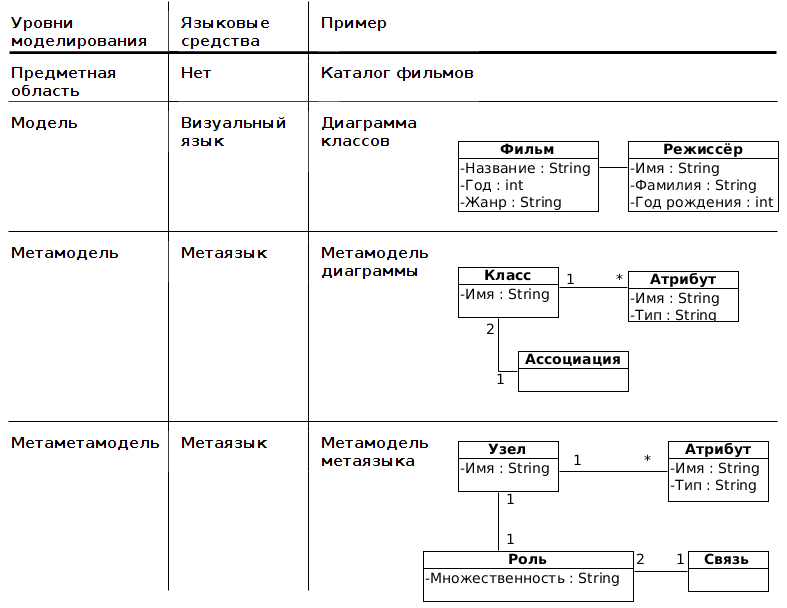
\includegraphics[width=0.85\textwidth]{images/presentation/metalevels.png}
    	\end{center}
    \end{figure}
\end{frame}

\begin{frame}
    \frametitle{Существующие модели жизненного цикла языка}
    \begin{itemize}
        \item M. Mernik et al., When and how to develop domain-specific languages
        \item D. Koznov, Process Model of DSM Solution Development and Evolution 
            for Small and Medium-Sized Software Companies
        \item A. Repenning, et al., Agentsheets: A medium for creating 
            domain-oriented visual languages
    \end{itemize}
\end{frame}

\begin{frame}
    \frametitle{Существующие DSM-платформы}
    \framesubtitle{Наличие визуальных языков для задания инструментальных средств}
    \begin{table}[ht]
    \begin{scriptsize}
        \tabulinesep=0.9mm
        \vspace*{-0.30cm}
    	\begin{tabu} {| X[1.2 l p] | X[1.2 c p] | X[1 c p] | X[1.1 c p] | X[1 c p] | X[1 c p] |}
    		\tabucline-
    		 Название                    & Метаредактор & Конкретный синтаксис & Ограничения & Трансфор-мации & Интерпре-тация \\
    		\tabucline-
    		\everyrow{\tabucline-}
    		MetaEdit+                    & Да           & Да                   & Нет         & ---           & ---           \\
    		Eclipse Modeling Project     & Да           & Да                   & Нет         & Нет           & Нет           \\
    		Generic Modeling Environment & Да           & Нет                  & Нет         & Да            & ---           \\
    		PSL/PSA                      & Нет          & ---                  & ---         & ---           & ---           \\
    		AToM3                        & Да           & Да                   & ---         & Да            & Да            \\
    		Microsoft Modeling SDK       & Да           & Нет                  & Нет         & ---           & ---           \\
    		Pounamu                      & Да           & Да                   & ---         & Нет           & ---           \\
    		DOME                         & Да           & Нет                  & ---         & Нет           & ---           \\
    		MetaLanguage                 & Да           & ?                    & ?           & ?             & ---           \\
    		\textbf{QReal}               & \textbf{Да}  & \textbf{Да}          & \textbf{Да} & \textbf{Да}   & \textbf{Да}
    		\label{tab:existingPlatformsCondensed}
    	\end{tabu}
    \end{scriptsize}
\end{table}\end{frame}

\begin{frame}
    \frametitle{<<Классическая>> методология разработки}
    \vspace*{-0.35cm}
    \begin{figure}
    	\begin{center}
    		\raisebox{0.4cm}{
        		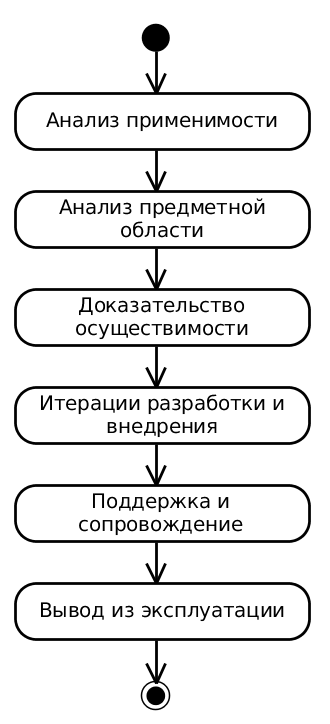
\includegraphics[width=0.20\textwidth]{images/presentation/classicalModel.png}
            }
    		\hspace{0.1cm}
    		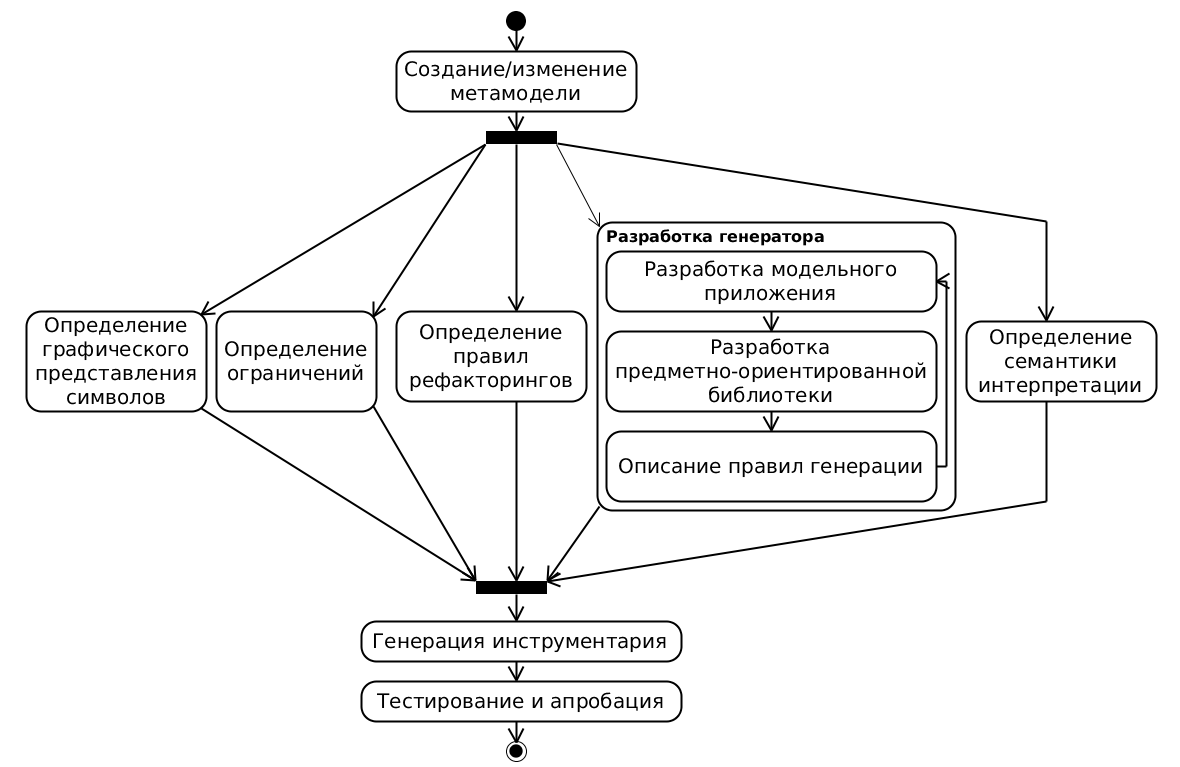
\includegraphics[width=0.75\textwidth]{images/presentation/classicalModelIteration.png}
    	\end{center}
    \end{figure}
\end{frame}

\begin{frame}
    \frametitle{<<Метамоделирование на лету>>}
    \begin{columns}[onlytextwidth]
       \begin{column}{0.6\textwidth}
         \begin{itemize}
             \item Создание визуального языка прямо в процессе рисования диаграммы, 
                 без метаредактора
             \item Быстрое прототипирование языка с непосредственным участием будущего пользователя
             \item Доработка созданного средства в ``классическом'' метаредакторе
         \end{itemize}
       \end{column}
       \begin{column}{0.3\textwidth}
            \begin{figure}
            	\begin{center}
            		\raisebox{0.4cm}{
                		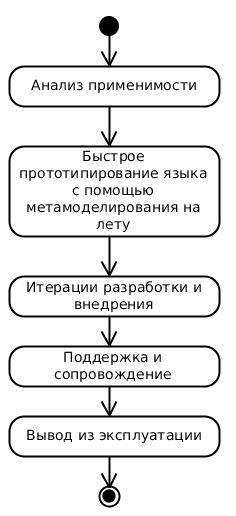
\includegraphics[width=0.9\textwidth]{images/presentation/metamodelingOnFly.png}
                    }
            	\end{center}
            \end{figure}
       \end{column}
​  \end{columns}
\end{frame}

\begin{frame}
    \frametitle{<<Метамоделирование на лету>>, особенности}
    \begin{itemize}
        \item Режим метамоделирования на лету скрывает от пользователя метамодель
        \begin{itemize}
            \item Интерпретация метамодели
            \item Пользовательский интерфейс, расширяющий обычный редактор диаграмм
            \begin{itemize}
                \item Добавление, удаление, редактирование внешнего вида и элементов и их свойств
            \end{itemize}
        \end{itemize}
        \item ``Бедность'' возможностей
        \begin{itemize}
            \item Отсутствие возможности задания синтаксических и семантических ограничений
            \item ``Плоская'' метамодель
            \item Разумные умолчания
        \end{itemize}        
    \end{itemize}
\end{frame}

\begin{frame}
    \frametitle{Реализация, компоненты системы QReal}
    \begin{figure}
        \begin{center}
      		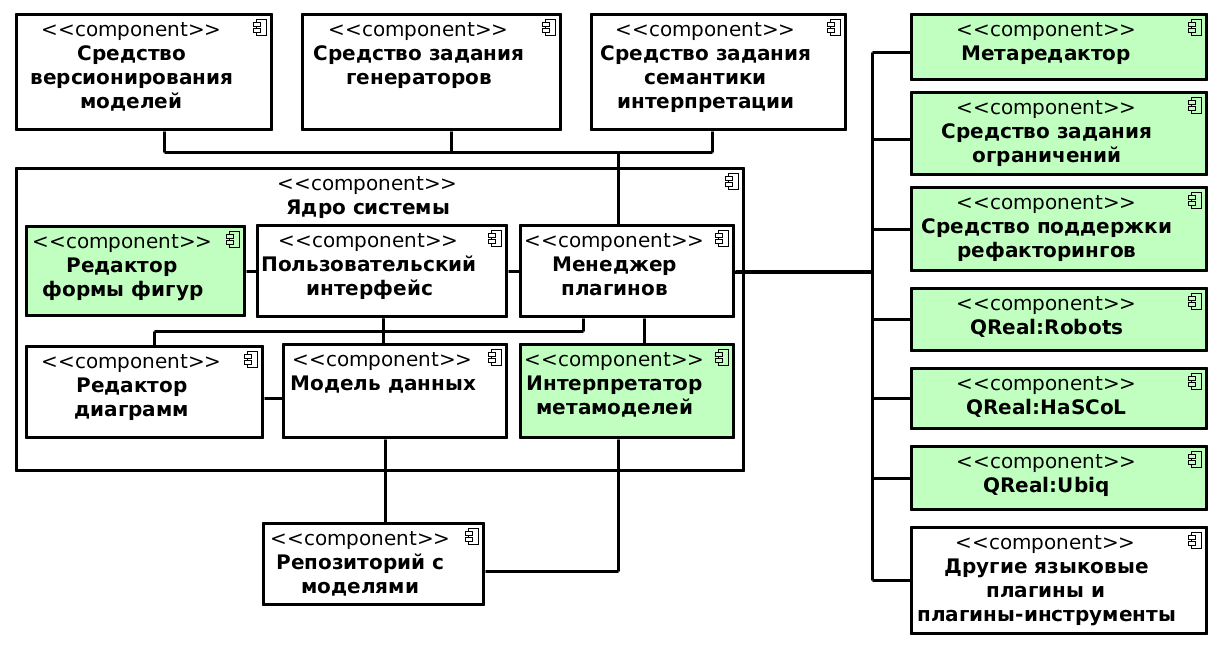
\includegraphics[width=\textwidth]{images/presentation/components.png}
        \end{center}
    \end{figure}
\end{frame}

\begin{frame}
    \frametitle{Метаредактор}
    \begin{figure}
        \begin{center}
      		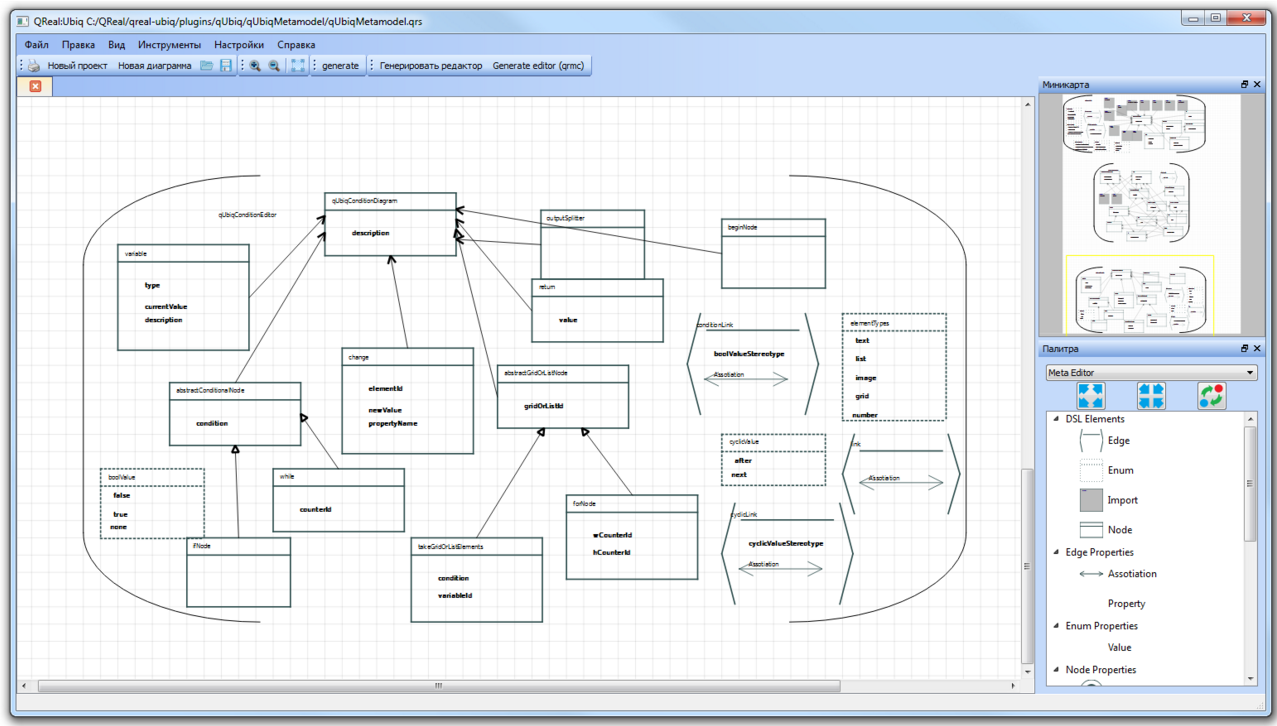
\includegraphics[width=\textwidth]{images/presentation/metaeditor.png}
        \end{center}
    \end{figure}
\end{frame}

\begin{frame}
    \frametitle{Редактор формы фигур}
    \begin{figure}
        \begin{center}
      		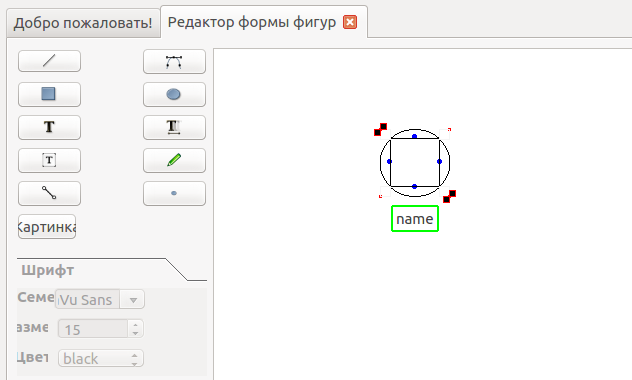
\includegraphics[width=0.8\textwidth]{images/presentation/shapeEditor.png}
        \end{center}
    \end{figure}
\end{frame}

\begin{frame}
    \frametitle{Редакторы ограничений и правил рефакторингов}
    \begin{figure}
        \begin{center}
      		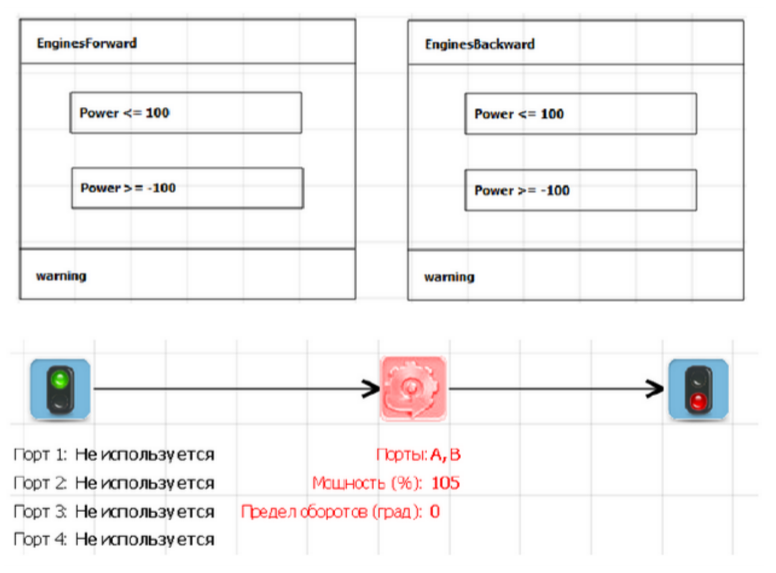
\includegraphics[width=0.5\textwidth]{images/presentation/constraints.png}
      		\hspace*{1cm}
      		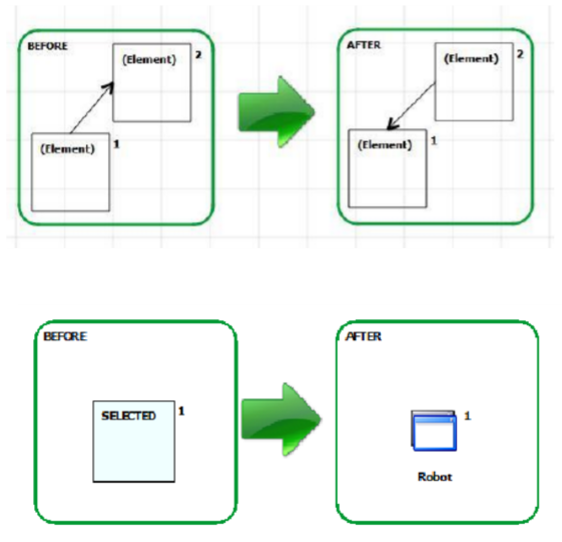
\includegraphics[width=0.4\textwidth]{images/presentation/refactorings.png}
        \end{center}
    \end{figure}
\end{frame}

\begin{frame}
    \frametitle{\large Реализация: <<метамоделирование на лету>>}
    \begin{figure}
       	\begin{center}
           	\raisebox{1cm}{
       	  		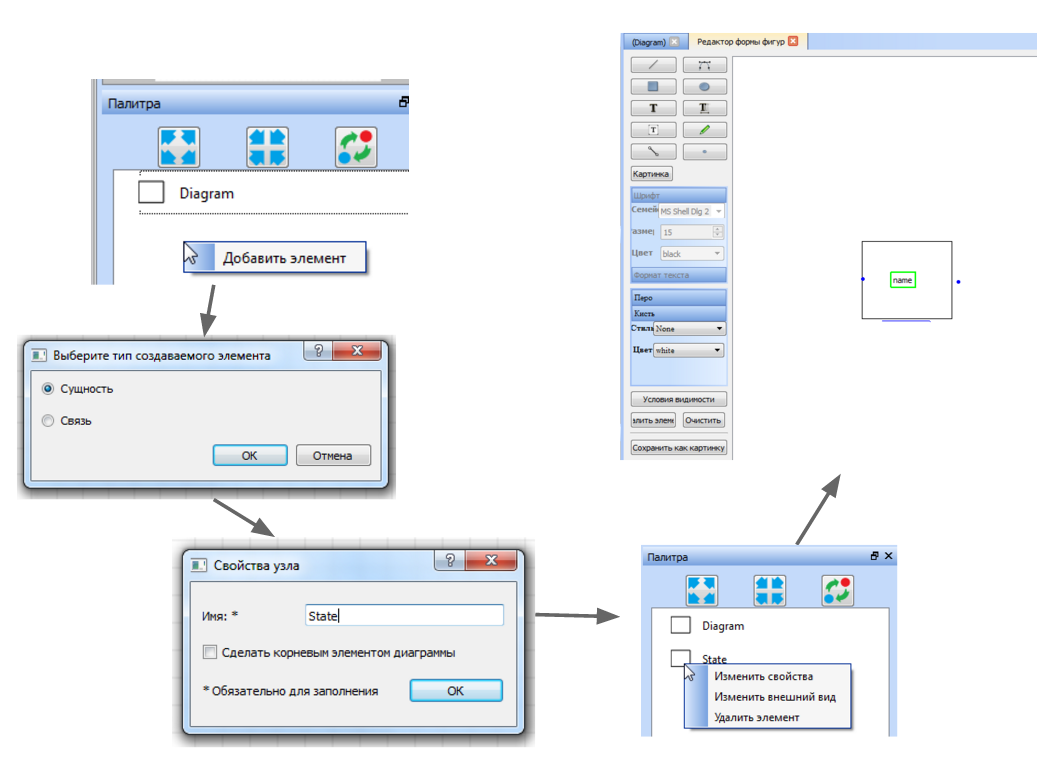
\includegraphics[width=0.8\textwidth]{images/presentation/metamodelingOnFlyImplementation.png}
       	  	}
       	\end{center}
    \end{figure}
\end{frame}

\begin{frame}
    \frametitle{Применение: QReal:Robots}
    \framesubtitle{Задача}
    \begin{columns}[onlytextwidth]
       \begin{column}{0.7\textwidth}
            \begin{itemize}
                \item Преподавание информатики с использованием исполнителя
                \item Робототехнические конструкторы
                \begin{itemize}
                    \item Lego Mindstorms NXT
                    \item Lego Mindstorms EV3
                    \item ТРИК
                \end{itemize}
                \item Средства визуального программирования
                \begin{itemize}
                    \item NXT-G
                    \item Robolab
                    \item Microsoft Robotics Developer Studio
                \end{itemize}
            \end{itemize}
        \end{column}
        \begin{column}{0.3\textwidth}
            \begin{figure}
            	\begin{center}
             		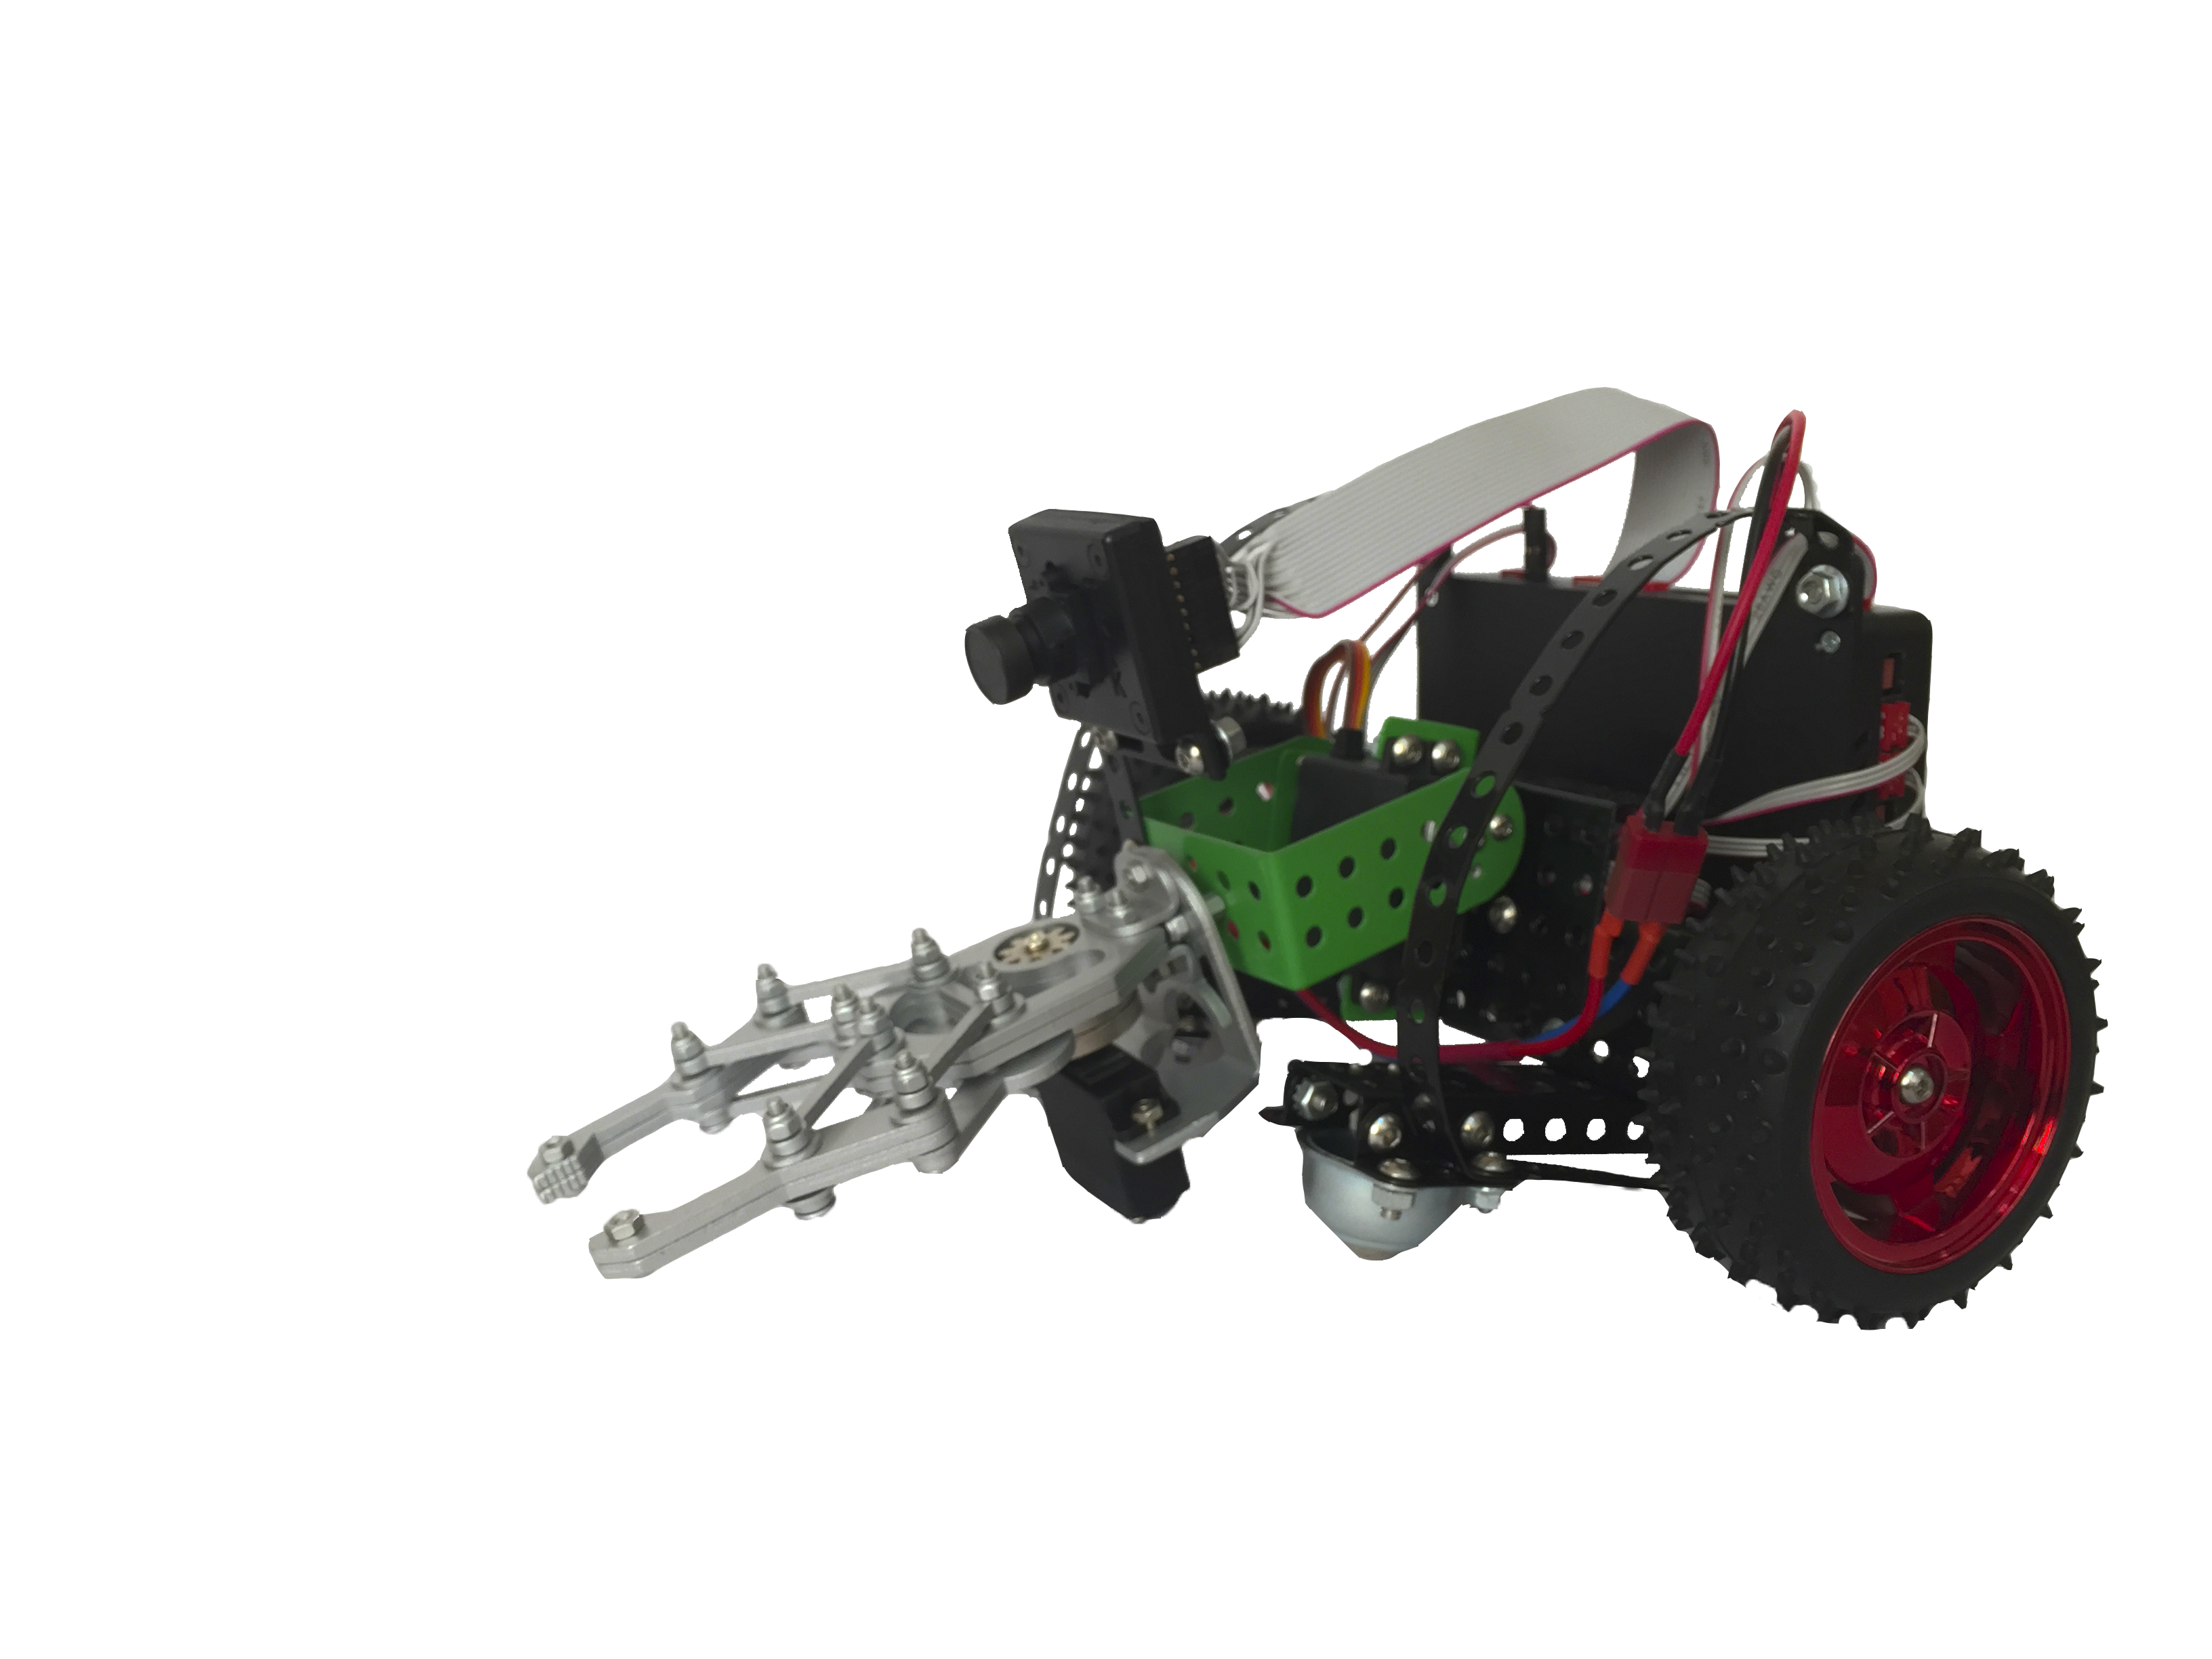
\includegraphics[width=\textwidth]{images/presentation/trik.png}\\
             		\hspace*{0.5cm}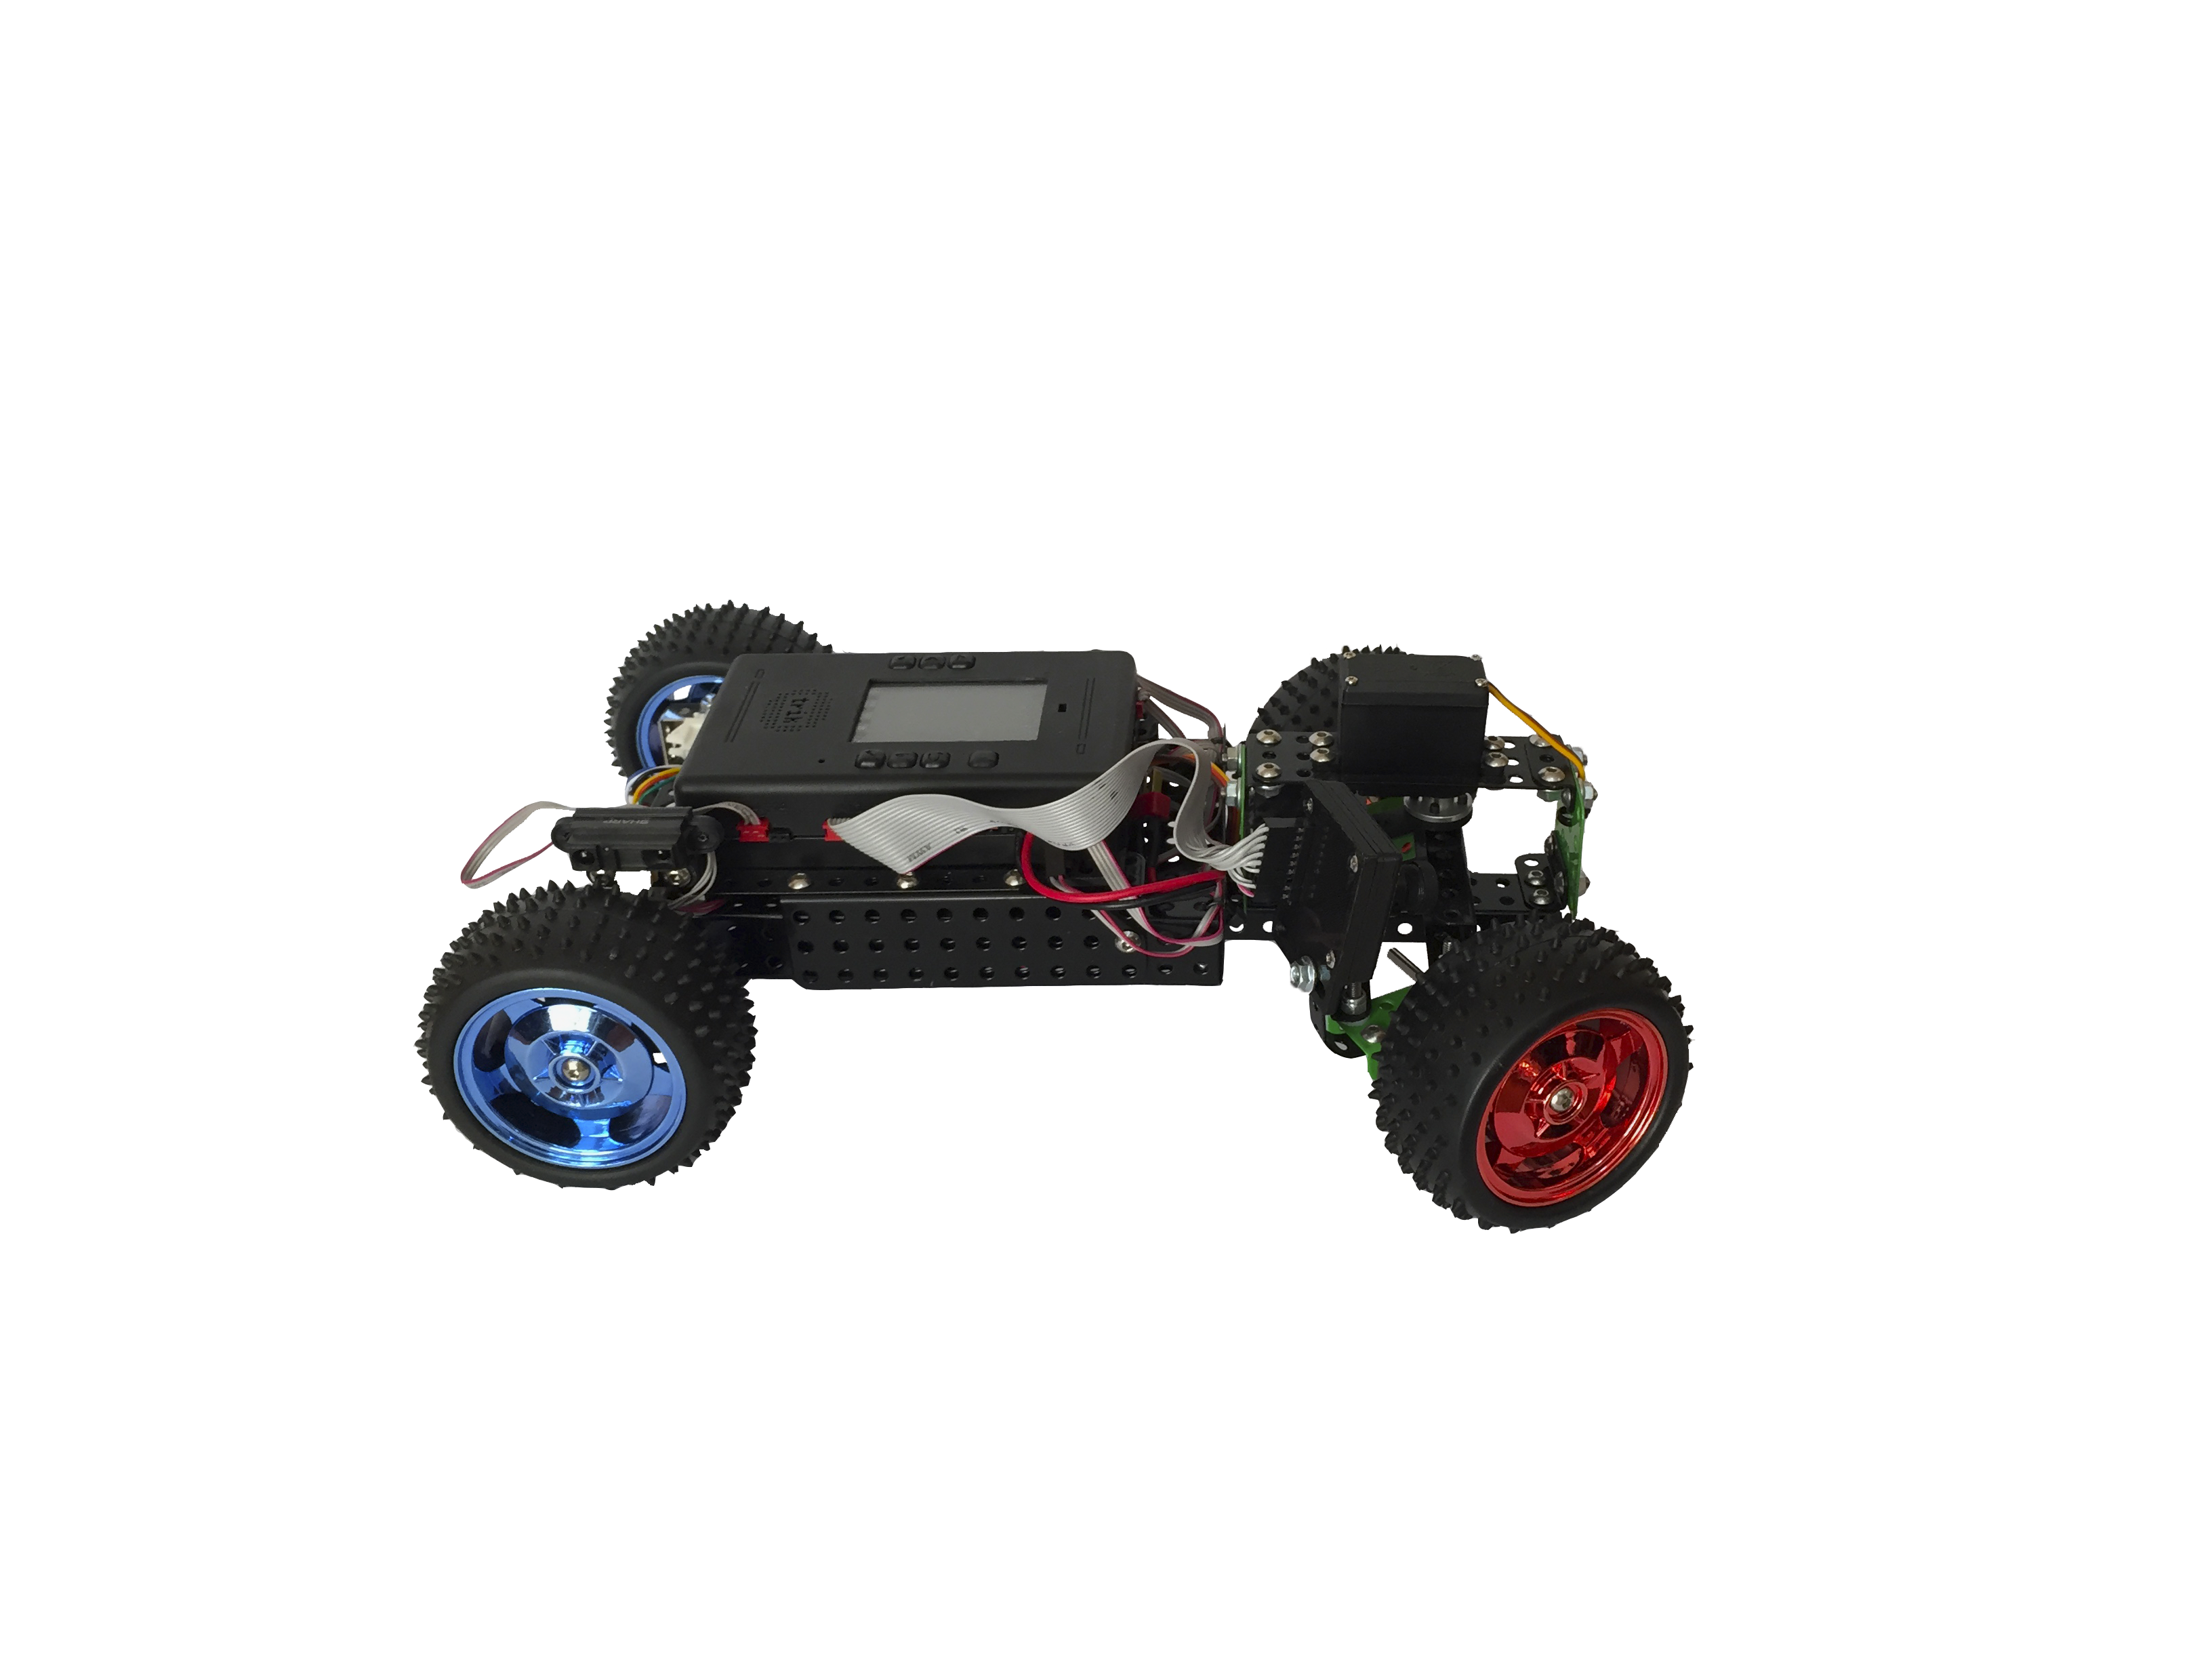
\includegraphics[width=\textwidth]{images/presentation/trik2.png}
            	\end{center}
            \end{figure}
        \end{column}
    \end{columns}
\end{frame}

\begin{frame}
    \frametitle{Применение: QReal:Robots}
    \framesubtitle{Визуальный язык}
    \begin{columns}[onlytextwidth]
       \begin{column}{0.5\textwidth}
            \begin{figure}
            	\begin{center}
             		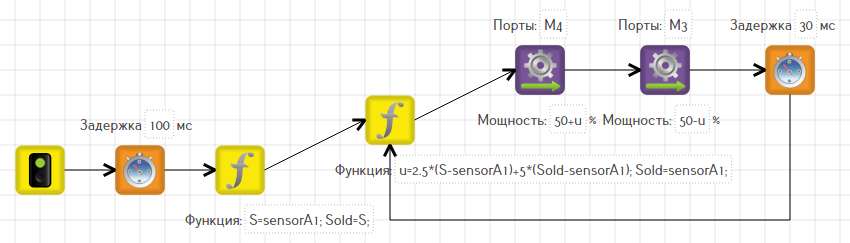
\includegraphics[width=\textwidth]{images/presentation/language1.png}\\
             		\vspace{0.5cm}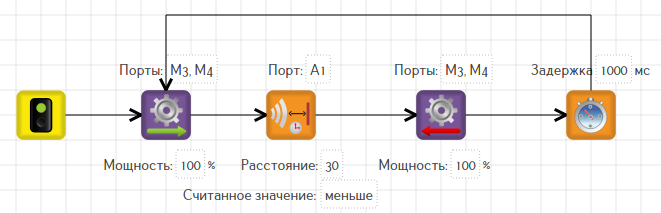
\includegraphics[width=\textwidth]{images/presentation/language2.png}\\
             		\vspace{0.5cm}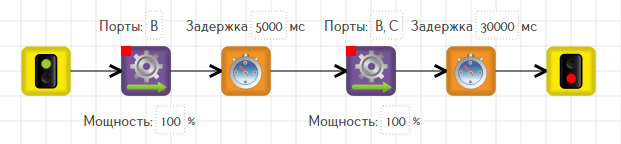
\includegraphics[width=\textwidth]{images/presentation/language4.png}
            	\end{center}
            \end{figure}
        \end{column}
        \begin{column}{0.5\textwidth}
            \begin{figure}
            	\begin{center}
             		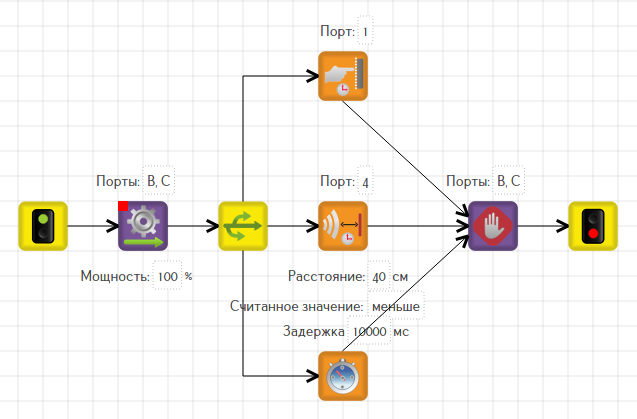
\includegraphics[width=0.9\textwidth]{images/presentation/language3.png}
            	\end{center}
            \end{figure}
        \end{column}
    \end{columns}
\end{frame}

\begin{frame}
    \frametitle{Применение: QReal:Robots}
    \framesubtitle{Метамодель}
    \begin{figure}
        \begin{center}
        	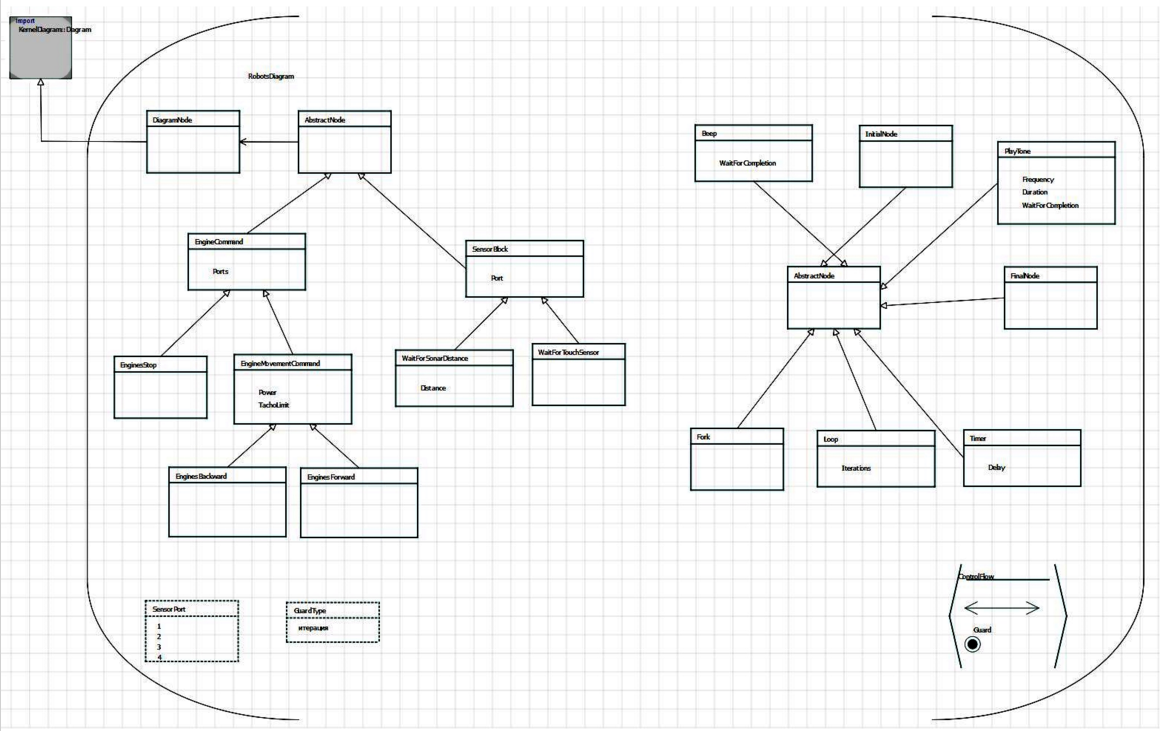
\includegraphics[width=0.9\textwidth]{images/presentation/robotsMetamodel.png}
        \end{center}
    \end{figure}
\end{frame}

\begin{frame}
    \frametitle{Применение: QReal:HaSCoL}
    \begin{columns}[onlytextwidth]
       \begin{column}{0.35\textwidth}
            \begin{figure}
            	\begin{center}
             		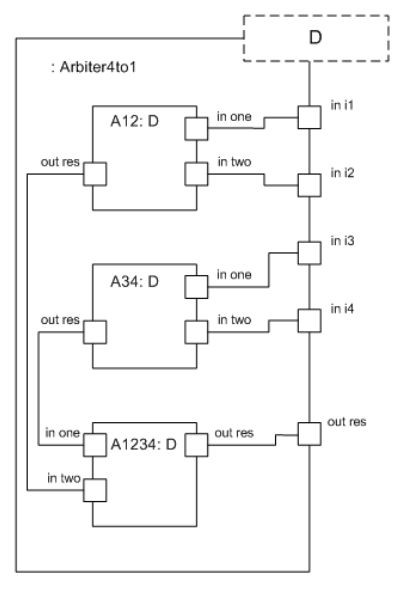
\includegraphics[width=0.8\textwidth]{images/presentation/hascol1.png}\\
            	\end{center}
            \end{figure}
        \end{column}
        \begin{column}{0.65\textwidth}
            \begin{figure}
            	\begin{center}
             		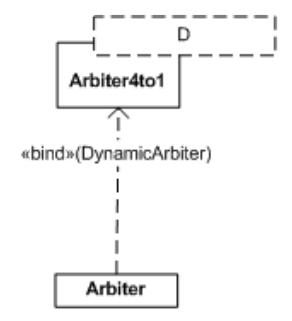
\includegraphics[width=0.25\textwidth]{images/presentation/hascol3.png}\\
             		\vspace{0.5cm}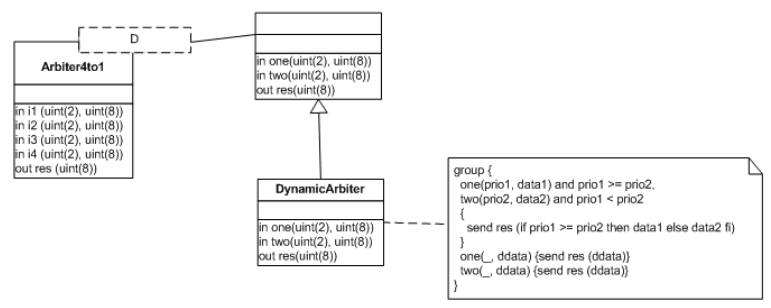
\includegraphics[width=\textwidth]{images/presentation/hascol2.png}
            	\end{center}
            \end{figure}
        \end{column}
    \end{columns}
\end{frame}

\begin{frame}
    \frametitle{Применение: QReal:Ubiq}
    \begin{figure}
       	\begin{center}
        	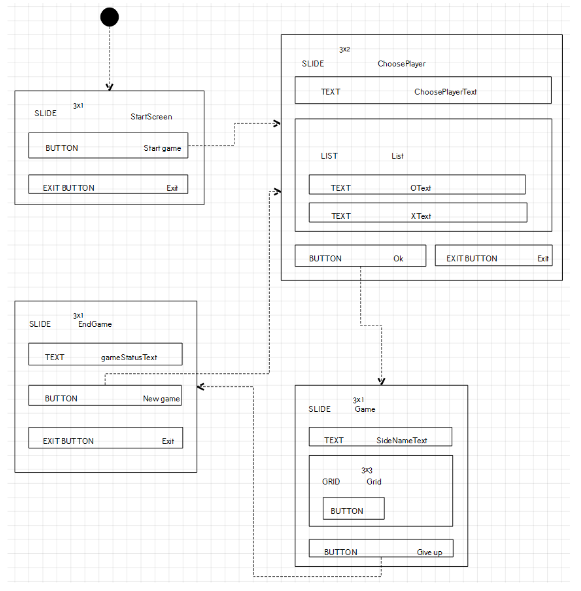
\includegraphics[width=0.6\textwidth]{images/presentation/ubiq.png}
       	\end{center}
    \end{figure}
\end{frame}

\begin{frame}
    \frametitle{Эксперимент}
    \framesubtitle{Сравнение скорости создания инструментов}
    \begin{table}[ht]
        \footnotesize
        \tabulinesep=0.9mm
    	\begin{tabu} {| X[1 l p] | X[1 l p] | X[1 l p] | X[1 l p] |X[1.1 l p] |}
    		\tabucline-
    		 Название DSM-платформы           & Редактор  & Генератор  & Ограничения  & Рефакторинги  \\
    		\tabucline-
    		\everyrow{\tabucline-}
    		MetaEdit+                         & 20 минут  & 30 минут   & ---          & ---           \\
    		Eclipse Modeling Project          & 2 часа    & 50 минут   & 17 минут     & 40 минут      \\
    		QReal (метаредактор)              & 15 минут  & 15 минут   & 10 минут     & 15 минут      \\
    		QReal (метамоделирование на лету) & 5 минут   & 15 минут   & ---          & ---
    		\label{tab:experiment}
    	\end{tabu}
    \end{table}
\end{frame}

\begin{frame}
    \frametitle{Публикации}
    \begin{itemize}
        \scriptsize
        \item \textbf{Литвинов, Ю.В. Реализация визуальных средств программирования роботов
            для изучения информатики в школах [Текст] / Ю.В. Литвинов // Компьютерные
            инструменты в образовании. --- 2013. --- No 1. --- С. 36--45.}
        \item \textbf{Литвинов, Ю.В. Средства быстрой разработки предметно-ориентированных
            решений в metaCASE-средстве QReal [Текст] / А.С. Кузенкова, А.О. Дерипаска, 
            К.С. Таран, А.В. Подкопаев, Ю.В. Литвинов, Т.А. Брыксин 
            // Научно-технические ведомости СПбГПУ. Информатика. Телекоммуникации.
            Управление. --- 2011. --- No 4 (128). --- С. 142--145.}
        \item \textbf{Литвинов, Ю.В. QReal: платформа визуального предметно-ориентированного
            моделирования [Текст] / А.Н. Терехов, Т.А. Брыксин, Ю.В. Литвинов 
            // Программная инженерия. --- 2013. --- No 6. --- С. 11--19.}
        \item \textbf{Y. Litvinov. QReal DSM platform-An Environment for Creation of
            Specific Visual IDEs [Text] / A. Kuzenkova, A. Deripaska, T. Bryksin, 
            Y. Litvinov, V. Polyakov 
            // ENASE 2013 --- Proceedings of the 8th International Conference on 
            Evaluation of Novel Approaches to Software Engineering. --- Setubal, Portugal : 
            SciTePress, 2013. --- P. 205--211.}
        \item Архитектура среды визуального моделирования QReal [Текст] / А.Н. Терехов,
            Т.А. Брыксин, Ю.В. Литвинов, К.К. Смирнов, Г.А. Никандров [и др.] 
            // Системное программирование. --- 2009. --- No 4. --- С. 171--196.
        \item Поддержка жестов мышью в мета-CASE-системах [Текст] 
            / М.С. Осечкина, Т.А. Брыксин, Ю.В. Литвинов, Я.А. Кириленко 
            // Системное программирование. --- 2010. --- No 5. --- С. 52--75.
    \end{itemize}
\end{frame}

\begin{frame}
    \frametitle{Результаты}
    \begin{itemize}
        \small
        \item Разработана методика для создания предметно-ориентированных визуальных
        языков с помощью визуального языка метамоделирования и других визуальных
        языков
        \item Предложен новый способ метамоделирования: <<метамоделирование на лету>>,
        позволяющий доопределять и изменять визуальный язык в процессе его
        использования
        \item Предложенные методики реализованы в виде технологии на базе системы
        QReal
        \item Проведена апробация разработанных методик и технологии при создании
        инструментальных средств среды программирования роботов QReal:Robots и
        других предметно-ориентированных решений
    \end{itemize}
\end{frame}

\end{document} 